\section{Результаты (3)}\label{section:dyck_1_1}

\subsection{Алгоритм для смешанного языка Дика}

Смешанный язык Дика $\cool{D}_i \odot \cool{D}_j$ является пересечением двух КС языков, а именно, $\cool{D}_i \odot \cool{D}_j = L_1 \cap L_2$, где $L_1 : S_1 ::= S_1 S_1~|~(_1 S_1 )_1~|~ \dots (_i S_1 )_i ~|~ \eps ~|~ [ ~|~ ]$ и $L_2 : S_2 ::= S_2 S_2~|~[_1 S_2 ]_1~|~ \dots [_j S_2 ]_j ~|~ \eps ~|~ ( ~|~ )$ (то есть двух языков Дика, которые игнорируют скобки второго типа). 

Однако КС-языки не замкнуты относительно пересечения: при нём получается конъюнктивный язык~\cite{Okhotin01}, задача достижимости для которого является алгоритмически неразрешимой~\cite{Hellings14}. Более того, она неразрешима уже для языка $\cool{D}_2 \odot \cool{D}_2$ даже на двунаправленных графах~\cite{Li21}. 

Однако задача достижимости для языка $\cool{D}_1 \odot \cool{D}_1$ на двунаправленных графах вполне разрешима, причём за полиномиально время.

В этой главе будет приведён улучшение алгоритма Ли и др.~\cite{Li21} решения этой задачи, основанное на идее пересечения языков.

\begin{note}

  Здесь и далее будем считать, что первый язык Дика~--- язык круглых ПСП ($\cool{D}_p : S ::= SS~|~(S)~|~\eps$), второй~--- язык квадратных ПСП ($\cool{D}_b : T ::= T~|~[T]~|~\eps$).
\end{note}

Заметим, что слово принадлежит $\cool{D}_p \odot \cool{D}_b$, тогда и только тогда, когда на любом его префиксе баланс обоих типов скобок неотрицателен, а конечный баланс равен нулю. Баланс строки будем записывать как $(p, b)$, где $p$~--- баланс круглых скобок, а $b$~--- квадратных.

Для решения понадобится следующий вспомогательный факт:

\begin{lemma}{Ли и др.~\cite{Li21}}\label{lm:dyck_6v}
  В двунаправленном графе, если между парой вершин $(u, v)$ существует какой-то $\cool{D}_1 \odot \cool{D}_1$ путь, то существует и такой путь, на котором в любой момент времени вложенность хотя бы одного типа скобок не превышает $6 |V|$.
\end{lemma}

\begin{figure}[h]
  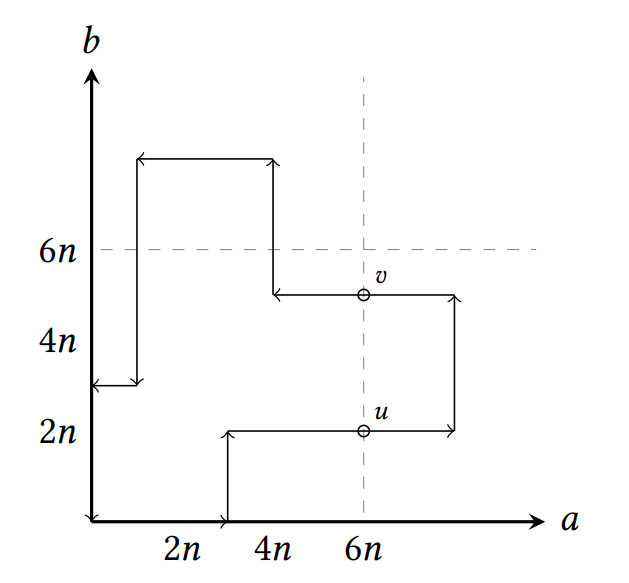
\includegraphics[width=0.75\linewidth]{img/6n_6n_path}
  \caption{Путь в координатах баланса}
  \label{img:6v_path}
\end{figure}

\TODO: картиночька

Нарисуем~(рис.~\ref{img:6v_path}) такой (как в утверждении леммы~\ref{lm:dyck_6v}) путь на плоскости, где первая координата~--- баланс круглых скобок, вторая~--- баланс квадратных (т.е. просто $p$ и $b$). Тогда во-первых, весь путь будет проходить в первой четверти. Во-вторых, он не будет заходить (найдётся такой, что не будет заходить, и мы ищем именно его) в сектор $[6|V|+1, +\oo) \times [6|V|+1, +\oo)$
    
То есть путь можно искать следующего вида: он в основном ходит внутри квадрата $[0, 6|V|] \times [0, 6|V|]$, иногда выходя из него, но только по одной координате (т.е. либо в сектор $[0, 6|V|] \times [6|V| + 1, +\oo)$, либо в сектор $[6|V| + 1, +\oo) \times [0, 6|V|]$).

Тогда можно искать отдельно две эти сущности: куски путей внутри квадрата $[0, 6|V|] \times [0, 6|V|]$, и куски путей снаружи.

% Т.е. нужно разобрать отдельно две сущности: куски путей внутри квадрата, и куски путей, которые выходят погулять.

Вооружившись этим знанием, построим алгоритм:

\begin{enumerate}
    \item {\bf Часть пути, лежащая в квадрате $\mathbf{[0, 6|V|] \times [0, 6|V|]}$}

    Внутри квадрата ограничена вложенность обоих типов скобок. Помним из прошлой главы (замечание~\ref{fact:regular_cfpq}), что в случае ограниченной вложенности язык получается регулярным. Строим автоматы для таких регулярных языков: $\cool{D}_p^{6|V|}$ и $\cool{D}_b^{6|V|}$, оба размера $\O(n)$.

    Пересекая оба этих языка и входной граф получаем автомат, состояние в котором~--- тройка $\q{v, p, b}$ (вершина и два баланса). Размер автомата: $\O(|V|^3)$ вершин, $\O(|E||V|^2)$ рёбер.

    Также в этом автомате нужно провести $\eps$-рёбра, соответствующие путям, выходящим за границы квадрата. Такие пути идут из состояния $(u, 6|V|, b_1)$ в состояние $(v, 6|V|, b_2)$ (и аналогично для другого типа скобок). Таких рёбер может быть столько, сколько есть различных пар $(u, b_1)$/$v, b_2$, то есть $\O(|V|^4)$.

    % Помним (из прошлой главы), что если хотим решать $D_1$-достижимость, зная, что вложенность ограничена, можем это с помощью ДКА делать.

    % Макс <3
    \begin{figure}[h]
      \begin{tikzpicture}
        \node[state, initial, accepting](n0) {$0$};
        \node[state, right=of n0](n1) {$1$};
        \node[state, right=of n1](n2) {$2$};
        \node[state, right=6em of n2](n3) {$3$};
        \node[state, right=6em of n3](n4) {$6|V|$};

        \foreach \y [evaluate=\y as \ny using int(\y+1)] in {0,1} {
          \draw (n\y)  edge[bend left=15] node[above] {\tt (} (n\ny);
          \draw (n\ny) edge[bend left=15] node[below] {\tt )} (n\y);
        }

        \foreach \y [evaluate=\y as \ny using int(\y+1)] in {2,3} {
          \draw (n\y)  edge[bend left=15] node[above] {\tt (} (n\ny);
          \draw (n\ny) edge[bend left=15] node[below] {\tt )} (n\y);
        }


        \foreach \y  in {0,1,2,4} {
          \draw (n\y) edge[loop above] node{\tt [,]} (ny);
        }

        \node [thick, fill=white, shape=rectangle, minimum width=6em, minimum height=4em, anchor=center] at ([yshift=0em]n3) {$\dots$};
      \end{tikzpicture}
      \caption{Автомат для языка $\cool{D}_p^{6|V|}$}
      \label{img:dyck_6n_dfa}
    \end{figure}

    % Строим такие ДКА для обоих типов скобок. Т.к. и тот, и другой регулярный, то можем их прекрасно пересечь с нашим графом. 

    % Получается такой граф троек $(u, b, p)$ (вершина, баланс квадратных скобок, баланс круглых скобок) на $\O(n^3)$ вершинах и $\O(n^2 m)$ рёбрах.

    % Ещё в нём будут $\eps$-рёбра, найденные второй частью алгоритма. Эти рёбра имеют вид $(u, 6|V|, a) \to (v, 6|V|, b)$. Для всех возможных пар $a/b$ и $u/v$ их $\O(n^4)$.

    После этого нужно решить задачу достижимости для полученного графа-автомата. Покажем, что он получается неориентированным: из-за двунаправленности графа ребро $(u, b, p) \to (v, b+1, p)$ существует тогда и только тогда, когда и обратное ему. То же и с $\eps$-рёбрами: если есть путь, с балансом $(0, j-i)$, то есть и путь в обратную сторону с балансом $(0, i-j)$.

    В неориентированном графе выделяем компоненты связности, теперь из вершины $u$ есть $\cool{D}_p \odot \cool{D}_p$-путь, если $(u, 0, 0)$ и $(v, 0, 0)$ лежат в одной компоненте.

    Итого, эта часть алгоритма работает за dfs по графу-произведению, то есть за $\O(|V|^4)$.

    % Т.к. входной граф двунаправленный, то полученное произведение будет неориентированным (\textit{это не совсем тривиально, но понятно}), значит достижимость на нём можно искать просто dfs'ом за $\O(n^4)$.

    \item {\bf Часть пути, лежащая в $\mathbf{[0, 6|V|] \times [6|V| + 1, +\oo)}$}

    % В какой момент пути идут гулять? Когда вложенность одной из скобок ровно $6|V|$. А когда возвращаются? Тоже когда ровно $6|V|$. А во все моменты между $\ge 6|V|$. 

    % То есть хотим искать такие пути, что по одной скобке они просто сбалансированы ($6|V| \path 6|V|$), а по другой какие попало, но всё время не больше $6|V|$ ($a \path b$, $a, b \le 6|V|$). 

    Опять-таки, решаем через пересечение языков. Первый~--- наш граф ($L_1$). Второй~--- просто язык Дика ($L_2$) (опять-таки с оговорками про то, что скобочка другого типа~--- это то же, что и $\eps$). Третий~--- пути Дика, начинающиеся в балансе $a$ и заканчивающиеся в балансе $b$ ($L_3$) (решаем для всех возможных пар балансов, чтобы рёбра провести). Давайте решать отдельно для каждого $a$, то есть нам нужен язык Диковых последовательностей со стартовым балансом $a$, таких, что их баланс не уходит в минус. Язык, опять-таки регулярный. 

    Дальше пересекаем. Сначала пересекаем $L_1 \cap L_2$. Это просто прямое произведение~--- граф пар $(u, b)$ (для каждого $a$ отдельно, снаружи всего это как бы фор по $a$). Вершин в нём $\O(n^2)$, рёбер $\O(n m)$. Теперь нужно это ещё пересечь с $L_3$. Ну так это же просто язык Дика, а Дикову достижимость мы за $\O(m^{*} \alpha)$ на двунаправленных графах решаем (а произведение $L_1 \cap L_2$ как раз двунаправленное). 

    \TODO: допереписать

    Получаем $\O(n \cdot n m^{*} \alpha) = \O(n^4 \alpha)$.

\end{enumerate}

\subsection{Выводы и результаты по главе}